% Pinocchio-EP: Standard 140-2023 conformance and engineering practice report
% Compile: pdflatex main && pdflatex main   (IEEEtran class; available on Overleaf / TeX Live / MiKTeX)
\documentclass[conference,10pt]{IEEEtran}
\IEEEoverridecommandlockouts
\usepackage[T1]{fontenc}
\usepackage{graphicx}
\usepackage{booktabs}
\usepackage{array}
\usepackage{xcolor}
\usepackage{cite}
\usepackage[caption=false,font=footnotesize]{subfig}
\usepackage{url}
\usepackage[hidelinks]{hyperref}
\newcommand{\code}[1]{\texttt{\footnotesize #1}}
\definecolor{ok}{HTML}{0ca30c}
\newcommand{\pass}{\textcolor{ok}{\textbf{Pass}}}
% UI figure helper: shows the screenshot if present, else a framed placeholder (so the paper always compiles)
\newcommand{\uifig}[3]{%
  \begin{figure}[!t]\centering
  \IfFileExists{figures/ui/#1}{\includegraphics[width=\columnwidth]{figures/ui/#1}}%
    {\fbox{\parbox[c][3cm][c]{0.9\columnwidth}{\centering\footnotesize screenshot \code{#1}}}}
  \caption{#2}\label{#3}\end{figure}}

\begin{document}

\title{
\includegraphics[height=1.15cm]{figures/ergo-logo.png}\\[6pt]
Pinocchio-EP and ANSI/ASHRAE Standard 140-2023:\\ Conformance Testing and Engineering Practice}

\author{\IEEEauthorblockN{ERGO Energy LLP --- Pinocchio-EP Engineering}
\IEEEauthorblockA{Release \code{1.0.0+e2c8ebf} $\cdot$ EnergyPlus 26.1.0-6f2e40d102\\
www.ergoenergy.in/pinocchio $\cdot$ 27 October 2026}}

\maketitle

\begin{abstract}
Pinocchio-EP is a web-based building energy modelling application that authors EnergyPlus models through a guided
interface and runs an unmodified EnergyPlus~26.1 engine. ANSI/ASHRAE Standard~140-2023 treats the interface and the
engine together as the software under test. We therefore tested the released Pinocchio-EP build itself:
\begin{itemize}
\item \textbf{scope:} every test section of the standard, Sections~6--13, including Addendum~a's hourly acceptance
criteria and Addendum~b's empirical ETNA tests;
\item \textbf{inputs:} ASHRAE's official accompanying weather files and output templates;
\item \textbf{build path:} every model built through Pinocchio-EP's own IDF writer.
\end{itemize}
All five graded test groups of Annex~A3 pass: 136 of 136 range cases are inside the acceptance ranges. For the four
constant-coefficient ETNA cases, modelled heater energy agrees with the measurements to within 0.03--0.33\,\%. We
describe the engineering practices behind this result: unmodified-engine provenance, no silent input
transformations, version stamping, standard-format reporting, regression gates, and bit-level parity with
openstudio-standards. We also list the limits that remain.
\end{abstract}

\begin{IEEEkeywords}
ASHRAE Standard 140, BESTEST, building energy simulation, software validation, EnergyPlus, empirical validation, ETNA
\end{IEEEkeywords}

\section{Introduction}
Standard~140~\cite{s140} is the method of test that energy codes and incentive programmes use to qualify simulation
software. It is required by ASHRAE~90.1-2022 \S12.4.1.4 and Appendices~C and~G~\cite{s901}, by green-building
rating systems built on 90.1, and by the US DOE \S179D qualified-software process~\cite{doe179d}. Its Annex~A3
contains a no-proxy rule: results obtained through one user interface cannot document another interface on the
same engine. A tool built on EnergyPlus must therefore be tested as itself.

This report presents the results for the released Pinocchio-EP build and the practices that support them. All
inputs, outputs, filled ASHRAE workbooks and modeller reports are archived with the release.

\section{The Standard and Its Addenda}
Class~I tests cover:
\begin{itemize}
\item weather processing (Section~6);
\item thermal fabric (Section~7);
\item ground coupling (Section~8);
\item cooling, heating and air-side equipment (Sections~9--11);
\item Addendum~b's empirical ETNA tests (Section~13).
\end{itemize}
Section~12 holds the Class~II tests for simplified tools.

Annex~A3 grades five test groups (Table~\ref{tab:groups}). Addendum~a~\cite{s140a} adds a time-series criterion to
the thermal-fabric groups: the hourly loads on 1~February and 14~July must exceed a Pearson correlation of 0.879
against the reference median curve, and must stay below a case-specific RMSE limit. Addendum~b~\cite{s140b} adds
six empirical cases from the guarded ETNA twin test cells~\cite{etna}. Their comparison against measured heater
energy is informative only; there is no pass/fail.

\section{Architecture and Engineering Practices}
\subsection{Engine Provenance}
The server writes the IDF produced in the browser verbatim and invokes the official NREL EnergyPlus~26.1.0 Linux
release~\cite{eplus}. The build is pinned by hash \code{6f2e40d102}, and the container build fails if the binary or
its version-transition programs are missing. The desktop test engine is the identical build. The engine is never
patched; engine defects are reported (Section~\ref{sec:limits}) rather than worked around in code.

\subsection{One Model, No Silent Transformations}
Every Pinocchio-EP step edits one structured IDF model, and the IDF the user downloads is exactly the IDF that runs.
This release removed three silent behaviours found in the first audit:
\begin{itemize}
\item imported files had their time step capped at 4 per hour;
\item a missing weather file was replaced by a default climate;
\item the site-exposure field never reached the model.
\end{itemize}
Numerical settings now pass through unchanged, and the Review step displays them. A requested but missing weather
file is an error. Every run reports the weather file it used.

\subsection{Faithful Inputs}
The interface can express the standard's inputs exactly:
\begin{itemize}
\item layered glazing with spectral-average pane properties (Fig.~\ref{fig:glz});
\item materials with exact conductivity, density, specific heat and absorptances;
\item constant convection coefficients (Fig.~\ref{fig:conv});
\item full-wall overhangs and full-height fins;
\item other-side-coefficient boundaries;
\item Kiva ground coupling~\cite{kiva};
\item DX performance maps fitted inside the application;
\item any EnergyPlus object, through an IDD-validated ``add object'' dialog (Fig.~\ref{fig:add}).
\end{itemize}
Weather in TMY3, TMY2, TMY or WYEC2 format is converted to EPW on import~\cite{tmy3}. The converter is validated
hour-by-hour against ASHRAE's own EPW files.

\subsection{Validation Profile}
An opt-in ``Standard~140 / validation'' profile applies the standard's test conditions, each documented with its
clause:
\begin{itemize}
\item no daylight saving time or holidays (5.1.1.1);
\item no latent removal by ideal loads (7.2.1.13);
\item interior solar distribution (7.2.1.12);
\item the specified terrain (7.2.1.9.1).
\end{itemize}
Normal projects keep realistic defaults. This separation prevents test-specific assumptions from leaking into design
work.

\subsection{Traceability and Reporting}
Each build carries a version identifier, \code{1.0.0+<git sha>}. It is shown in the interface and written into every
exported IDF, as Annex~A2 block~A requires. The application produces the Annex~A2 modeller report
(\code{S140outNotes}, blocks A--G) and fills ASHRAE's official output workbooks in place (Fig.~\ref{fig:res}).

\subsection{Verification Discipline}
\begin{itemize}
\item \textbf{Tests:} 992 automated front-end tests and 210 back-end tests pass on the tested build.
\item \textbf{Regression gate:} it reruns Cases~600 and 900 on the real engine and checks them against Annex~A3.
\item \textbf{GUI--agent equivalence:} every interface field is also exposed to the AI agent through a registry, and
a test proves that GUI and agent produce identical models.
\item \textbf{OpenStudio parity:} the HVAC emitter reproduces openstudio-standards~\cite{osstd} exactly. All 117
parity cases match, with 0 text or order differences across 32\,805 objects and a maximum difference of zero across
9\,014\,040 hourly meter values.
\item \textbf{Independence from reference answers:} no input or code was adjusted to match reference results, as
5.1.1.10 requires; each disclosed modelling choice is recorded in block~C.
\end{itemize}

\section{Test Method}
Every case is a Pinocchio-EP project or imported IDF, exported by the same \code{exportIdf} routine as the
interface's Run button and executed on the pinned engine. The Section~7 cases use only data the interface writes.
Inputs come from ASHRAE's official 140-2023 accompanying files~\cite{s140files} and the Addendum~b ETNA files.
Annex~A3 scoring is implemented in the application (\code{bestest.js}).

\section{Results}
\begin{table}[!t]\centering
\caption{Annex A3 Graded Test Groups}\label{tab:groups}
\begin{tabular}{@{}lccc@{}}\toprule
Test group & In range & Needed & Result\\\midrule
Thermal fabric, low mass & 34/34 & 30 & \pass\\
Thermal fabric, high mass & 28/28 & 25 & \pass\\
Cooling equipment (Sec.~9) & 14/14 & 12 & \pass\\
Heating equipment (Sec.~10) & 6/6 & 5 & \pass\\
Air-side HVAC (Sec.~11) & 54/54 & 48 & \pass\\\midrule
\textbf{Total} & \textbf{136/136} & & \textbf{5/5}\\\bottomrule
\end{tabular}\end{table}

\begin{figure}[!t]\centering
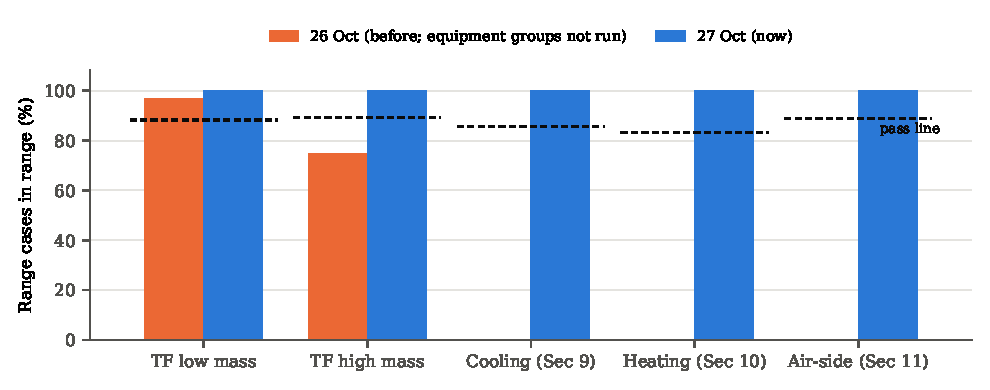
\includegraphics[width=\columnwidth]{figures/fig_groups.pdf}
\caption{Share of range cases in range per group, before the fixes (first audit) and for the tested release.}
\label{fig:groups}\end{figure}

\subsection{Thermal Fabric (Section 7)}
All 52 cases ran with no severe errors: 600--695, 900--995, 960, six free-float cases, and the in-depth cases
195--470, 800 and 810. Base results:
\begin{itemize}
\item Case~600: heating 4.301\,MWh, sensible cooling 6.015\,MWh;
\item Case~900: heating 1.661\,MWh, sensible cooling 2.506\,MWh.
\end{itemize}
All 22 Addendum~a day curves pass.

\subsection{HVAC Equipment (Sections 9--11)}
\begin{itemize}
\item \textbf{Cooling, CE100--CE200:} within 0.3--1.8\,\% of the quasi-analytical total energy.
\item \textbf{Cooling, CE300:} 35\,039\,kWh/yr, against a range of 33\,497--37\,023.
\item \textbf{Heating, HE100:} furnace input 77.756\,GJ against an analytical 77.713\,GJ.
\item \textbf{Heating, HE210:} 52.694\,GJ, against a range of 49.86--55.11.
\item \textbf{Air-side:} all 54 ranged quantities pass.
\end{itemize}

\subsection{Informative Sections}
\begin{itemize}
\item \textbf{Section~6:} the engine reproduces the weather file to $10^{-5}$, and 55 of 60 annual incident-solar
values fall inside the reference-program range.
\item \textbf{Section~8:} 16 of 17 cases ran with Kiva, within $-7.4$ to $+1.2$\,\% of the verified numerical
models.
\item \textbf{Section~12:} 38 of 58 results fall inside the informative example ranges.
\end{itemize}

\subsection{Empirical Validation (Section 13)}
\begin{itemize}
\item \textbf{Constant-coefficient cases:} modelled heater energy is within $+0.03$ to $+0.33$\,\% of measured
(Fig.~\ref{fig:etna}). Every best-steady-state hour lies inside the measurement uncertainty band.
\item \textbf{Automatic-convection cases (A3/B3):} $+0.77$ and $+1.04$\,\%, using the measured supply airflow as
specified.
\item \textbf{Time step:} for a model built from the specification, the result changes by less than 0.1\,\% between
4 and 60 steps per hour. The earlier import-path error in Fig.~\ref{fig:ts} is now removed.
\end{itemize}

\begin{figure}[!t]\centering
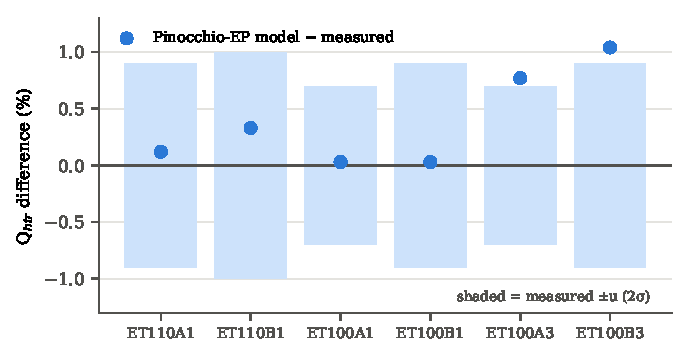
\includegraphics[width=0.92\columnwidth]{figures/fig_etna.pdf}
\caption{ETNA: modelled minus measured heater energy; the shaded band is the measured uncertainty $\pm u$ (2$\sigma$).}
\label{fig:etna}\end{figure}

\begin{figure}[!t]\centering
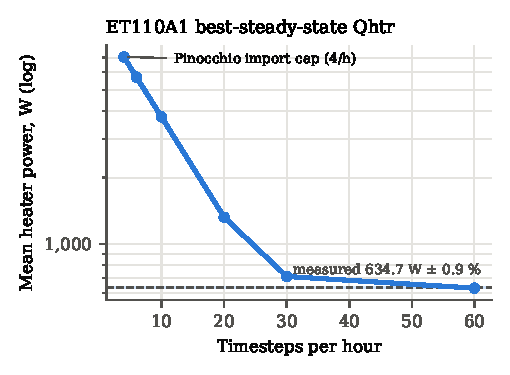
\includegraphics[width=0.78\columnwidth]{figures/fig_etna_timestep.pdf}
\caption{First audit: forcing an ETNA input to 4 steps/h changed heater power tenfold. The release keeps the
modeller's time step.}\label{fig:ts}\end{figure}

\section{User-Interface Evidence}
Figs.~\ref{fig:ui1} and~\ref{fig:ui2} show the released interface features that carry the standard's inputs and
outputs. Table~\ref{tab:map} maps each requirement to its implementation.

\begin{figure*}[!t]\centering
\subfloat[Project step: Std~140 profile, site exposure, TMY3 upload converted to EPW, ground reflectance.\label{fig:proj}]{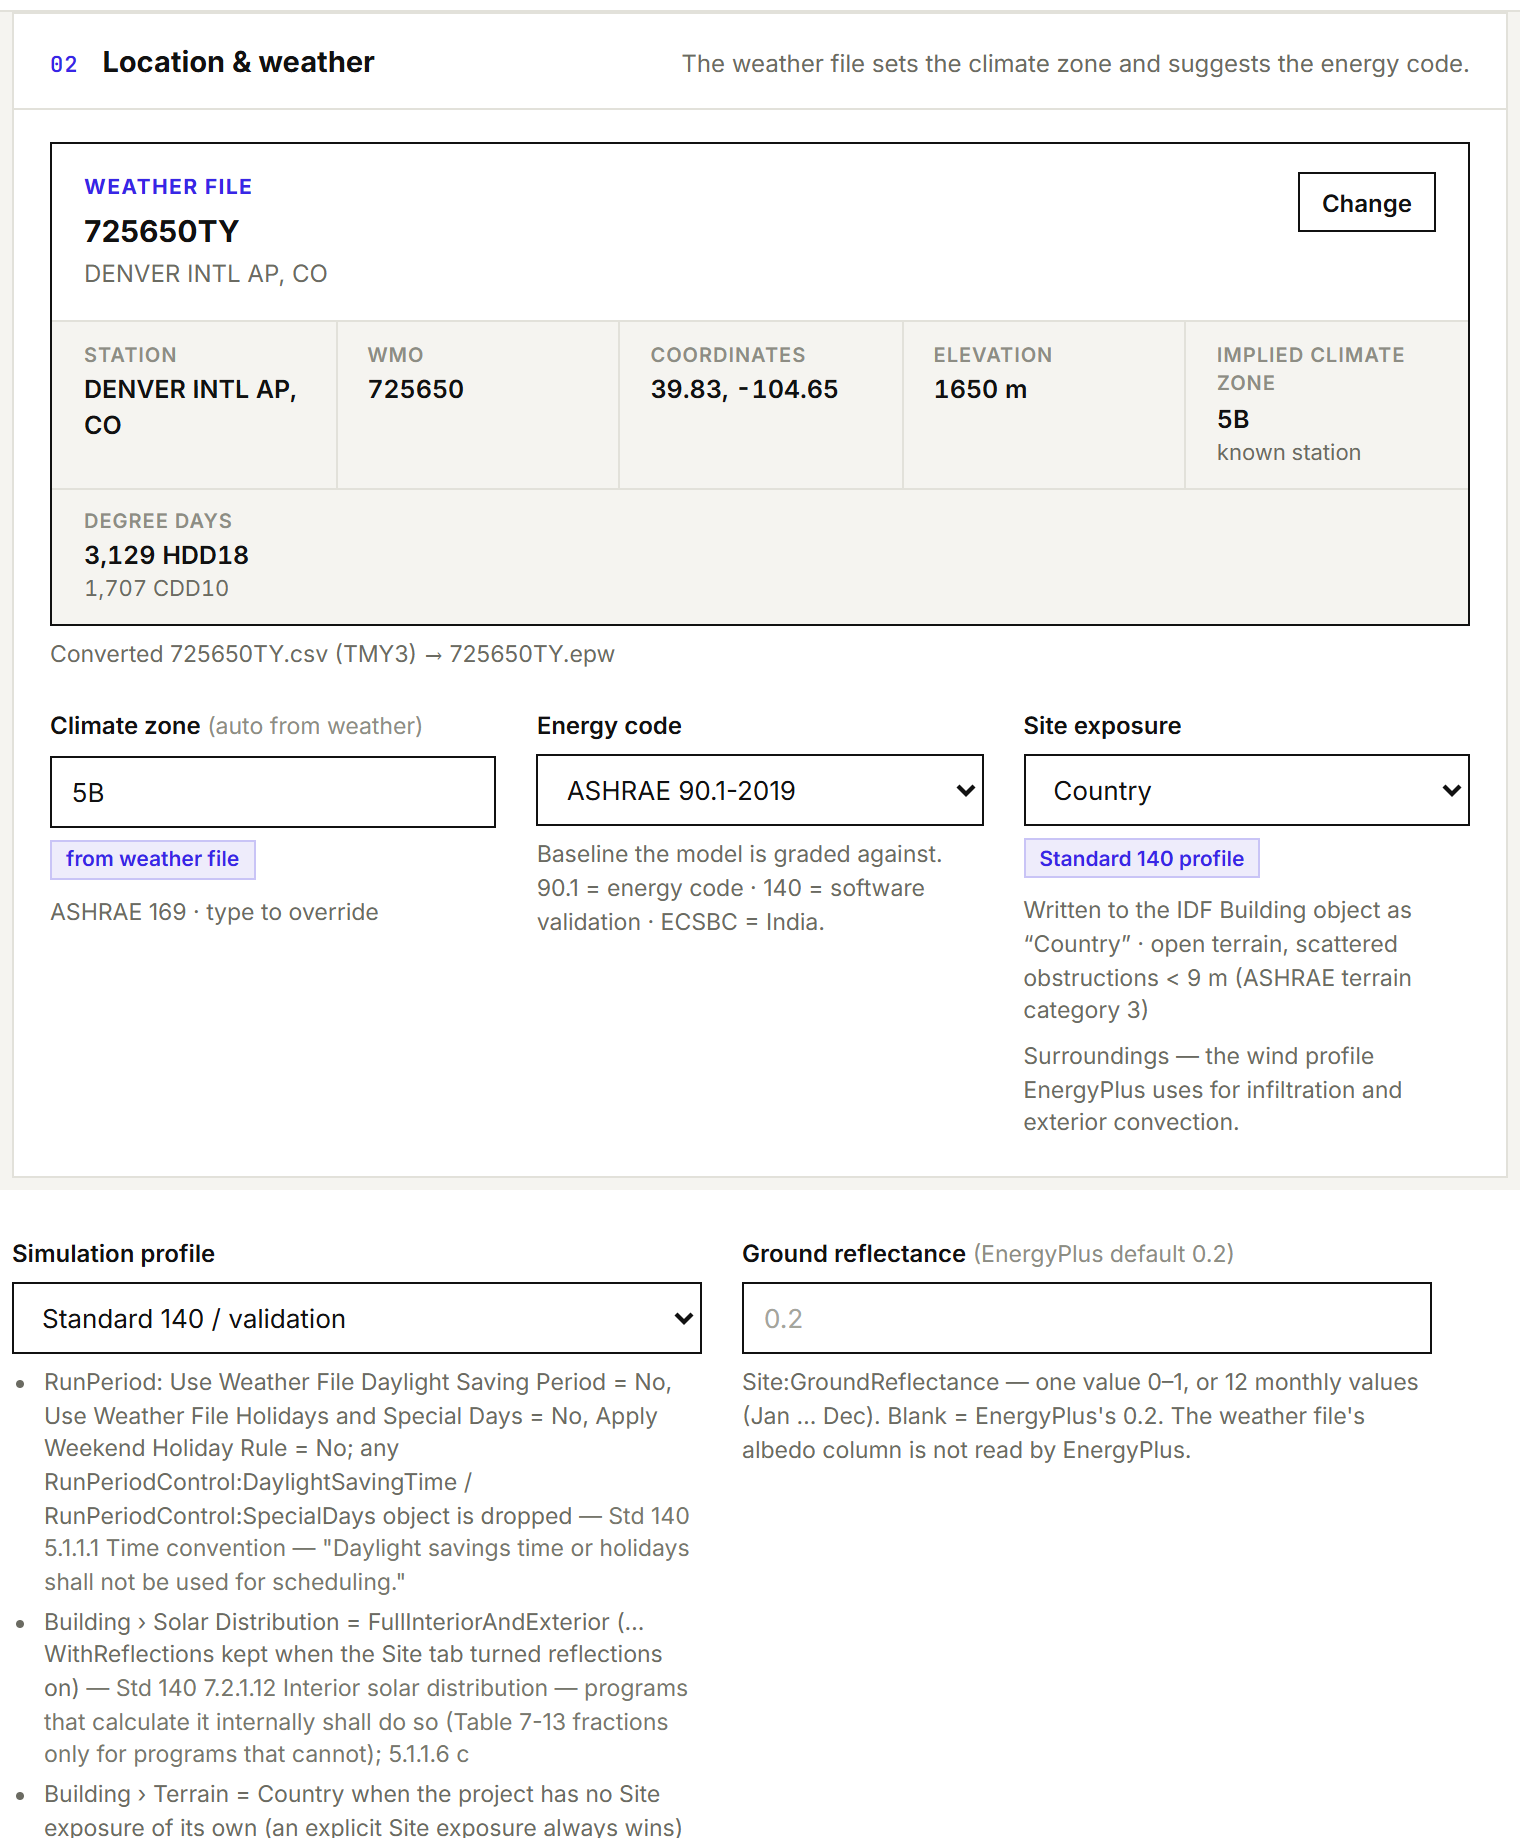
\includegraphics[height=6.4cm]{figures/ui/ui_project_std140.png}}\hfil
\subfloat[Layered glazing: Std~140 clear double pane; U and SHGC computed.\label{fig:glz}]{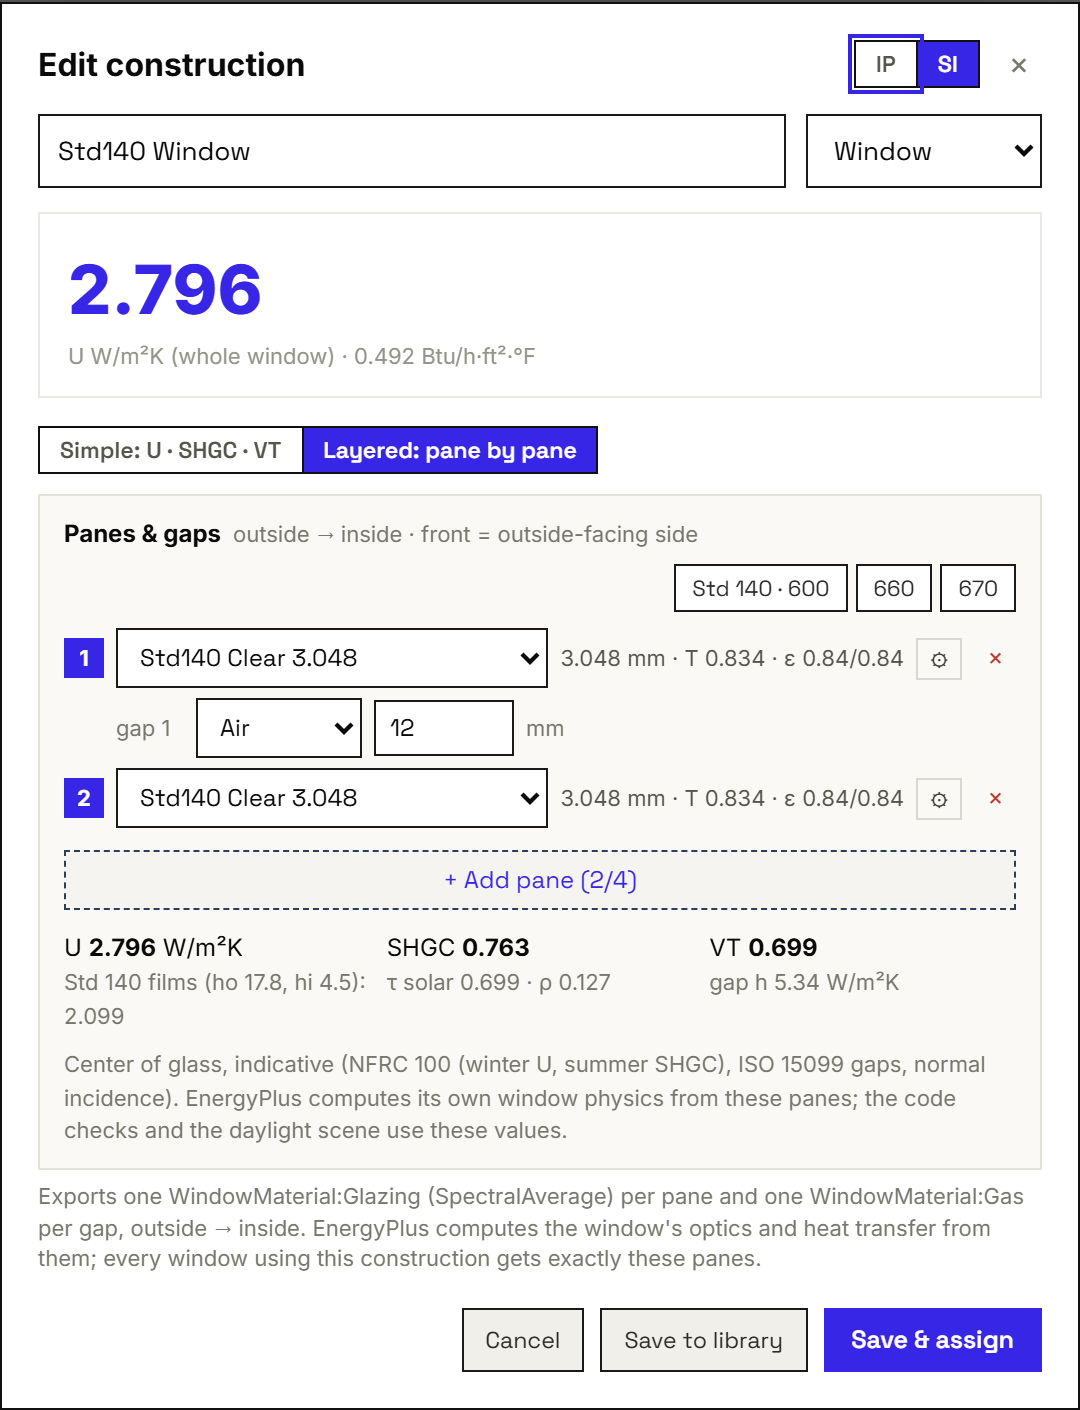
\includegraphics[height=6.4cm]{figures/ui/ui_glazing_layered.png}}\hfil
\subfloat[Exact material layers (Case~600 wall).\label{fig:mat}]{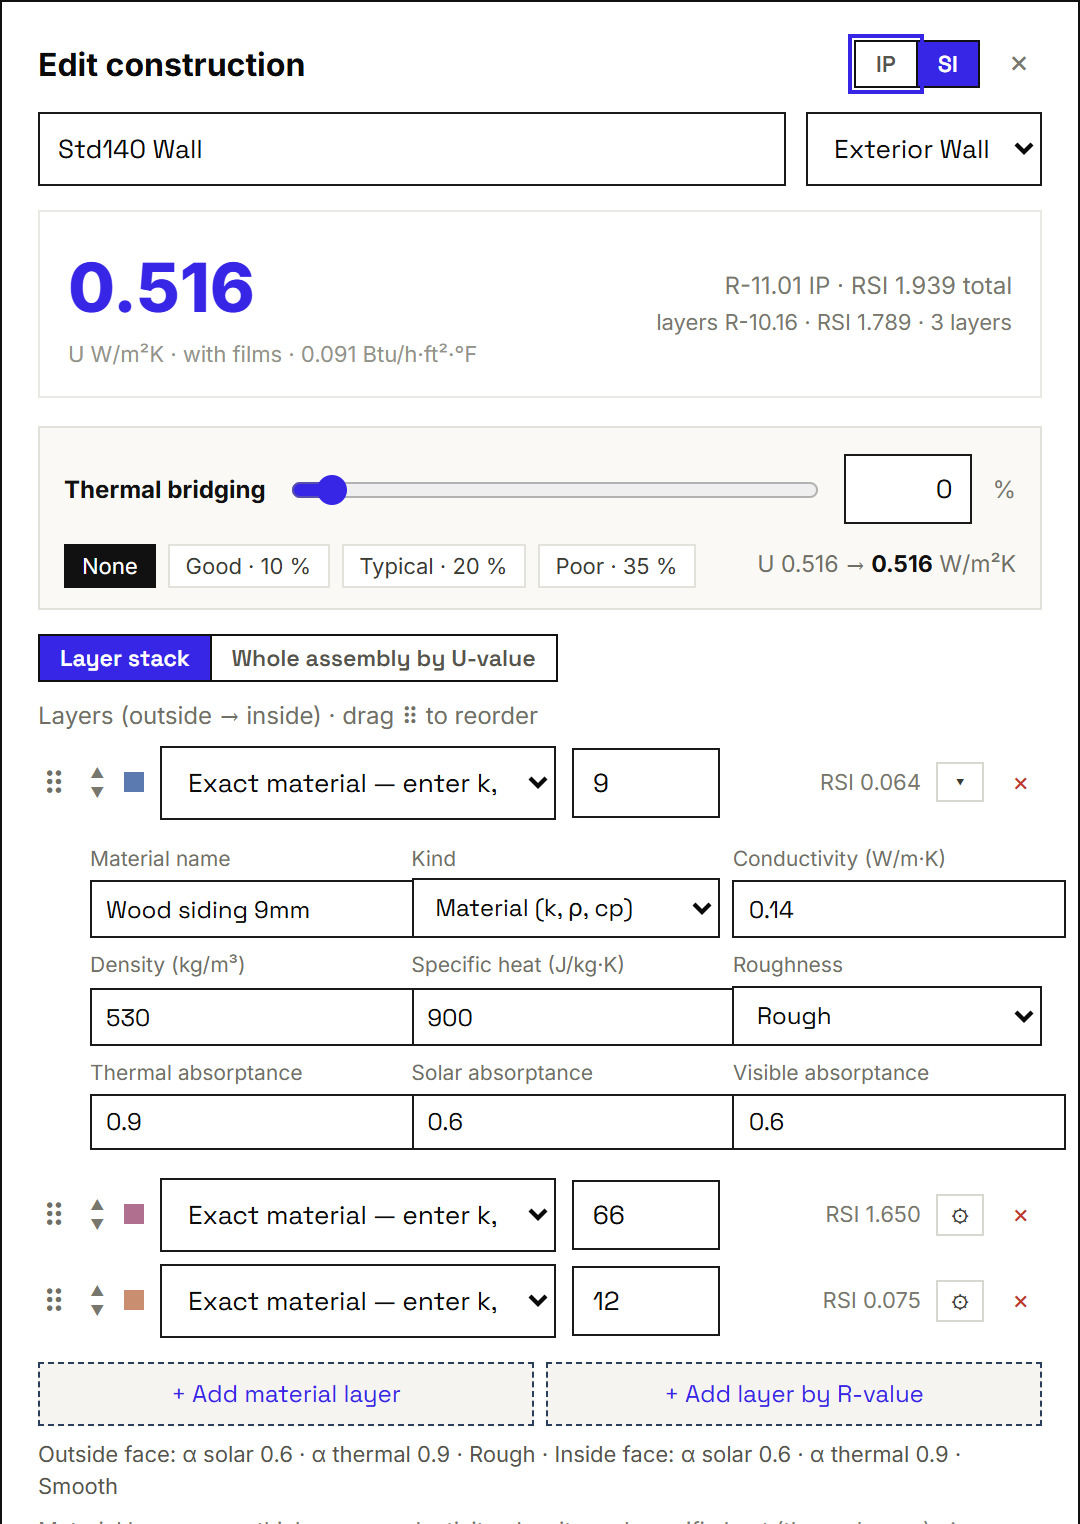
\includegraphics[height=6.4cm]{figures/ui/ui_materials_exact.png}}\\[2pt]
\subfloat[Surface heat transfer filled with Table~7-46 coefficients.\label{fig:conv}]{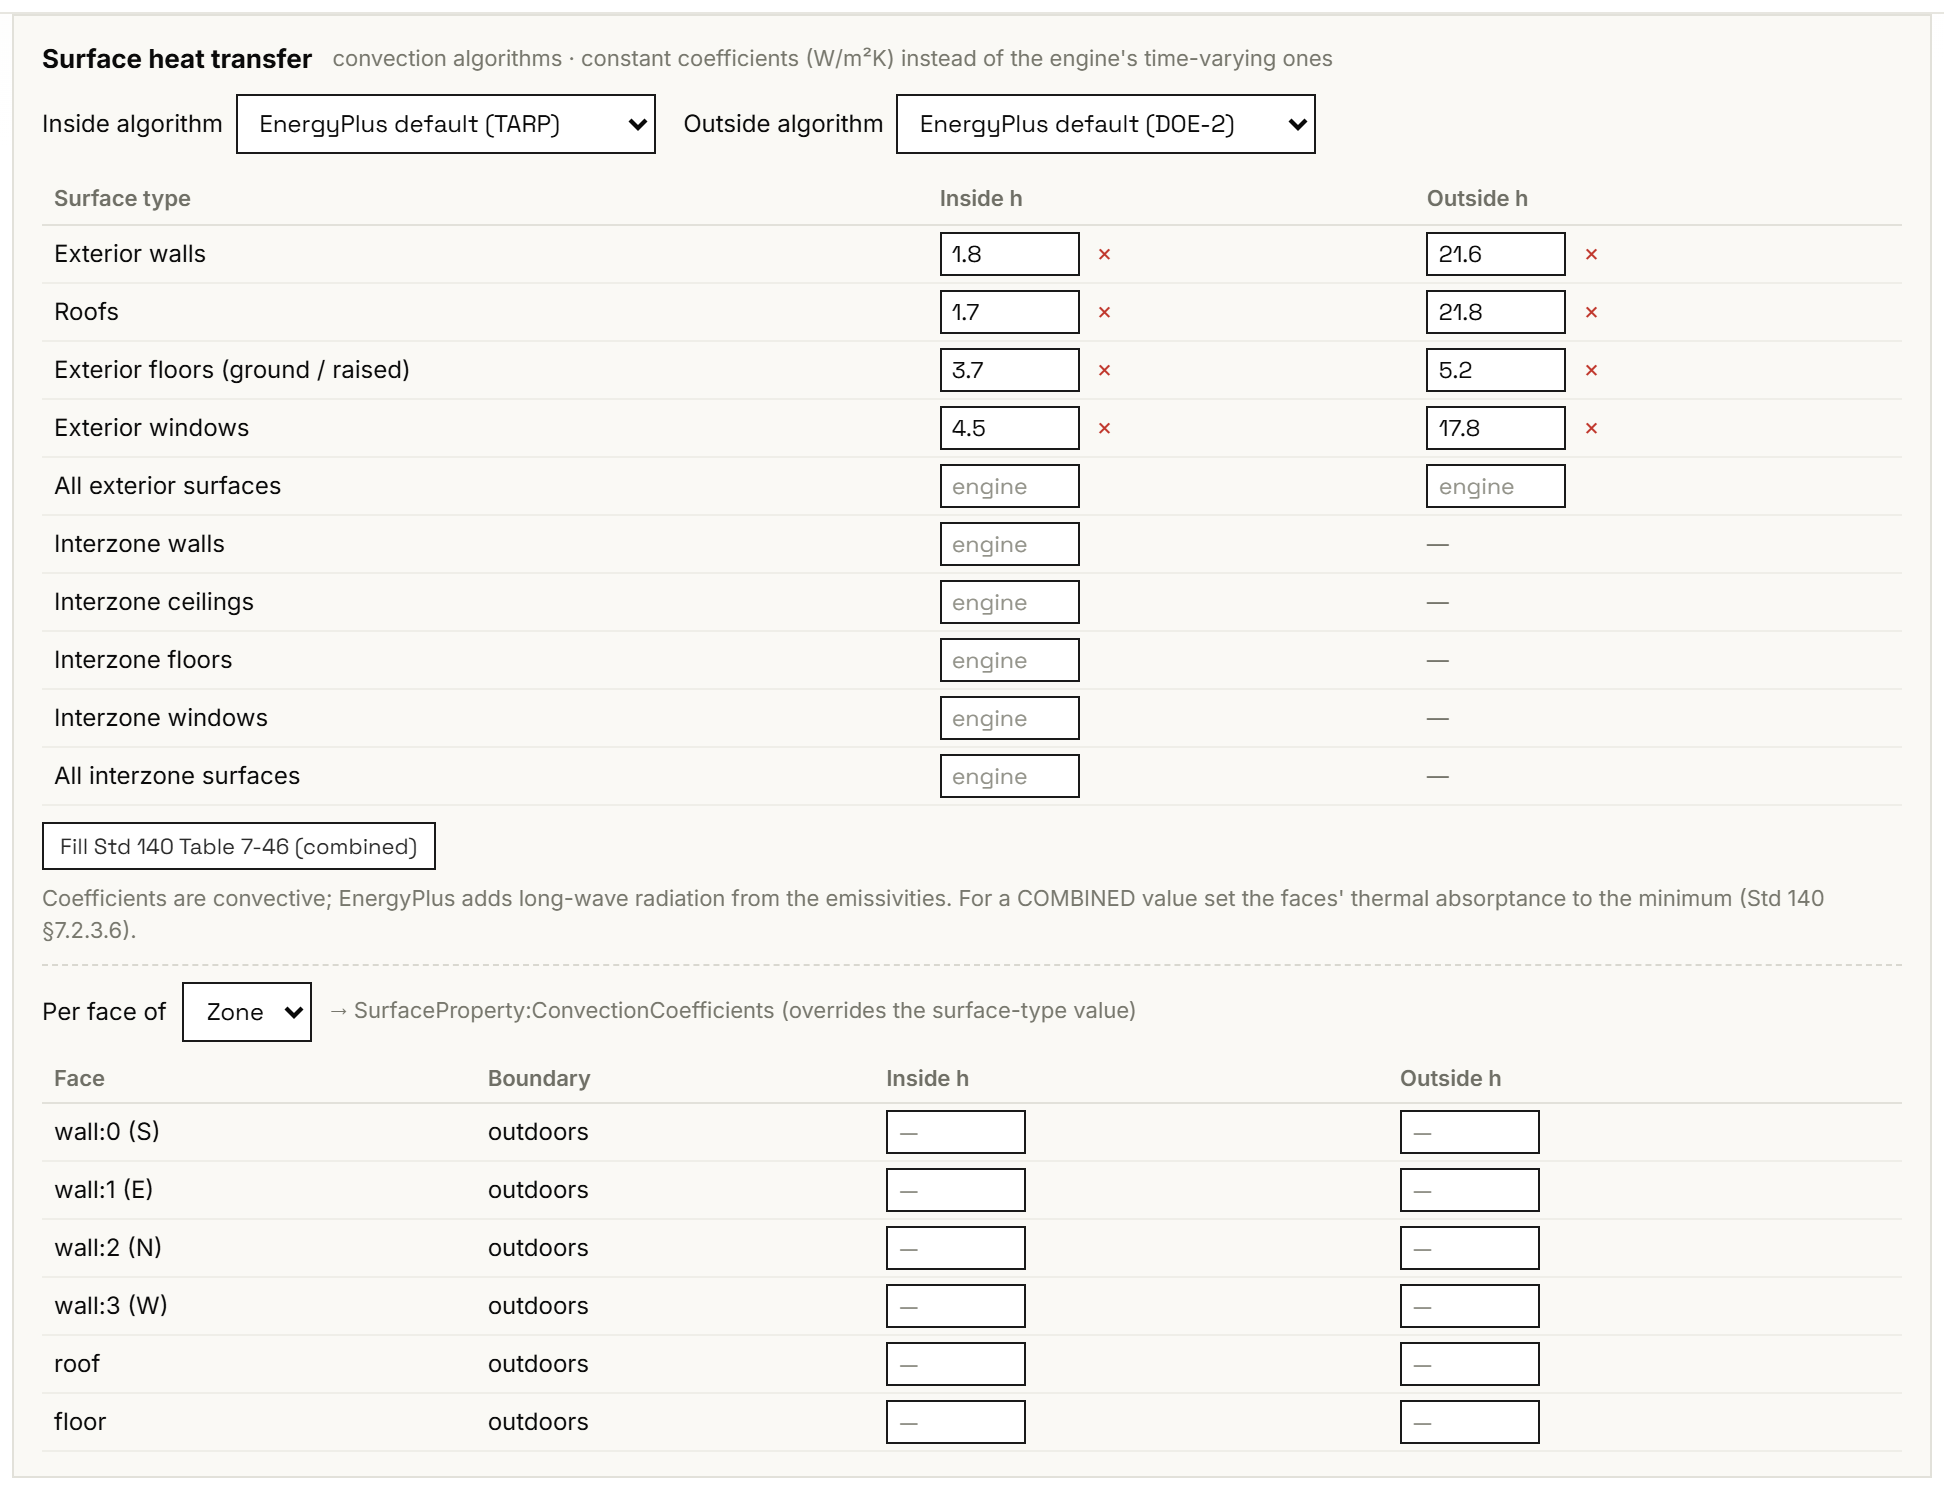
\includegraphics[height=4.1cm]{figures/ui/ui_convection.png}}\hfil
\subfloat[IDD-validated ``add object'' dialog (all 856 classes).\label{fig:add}]{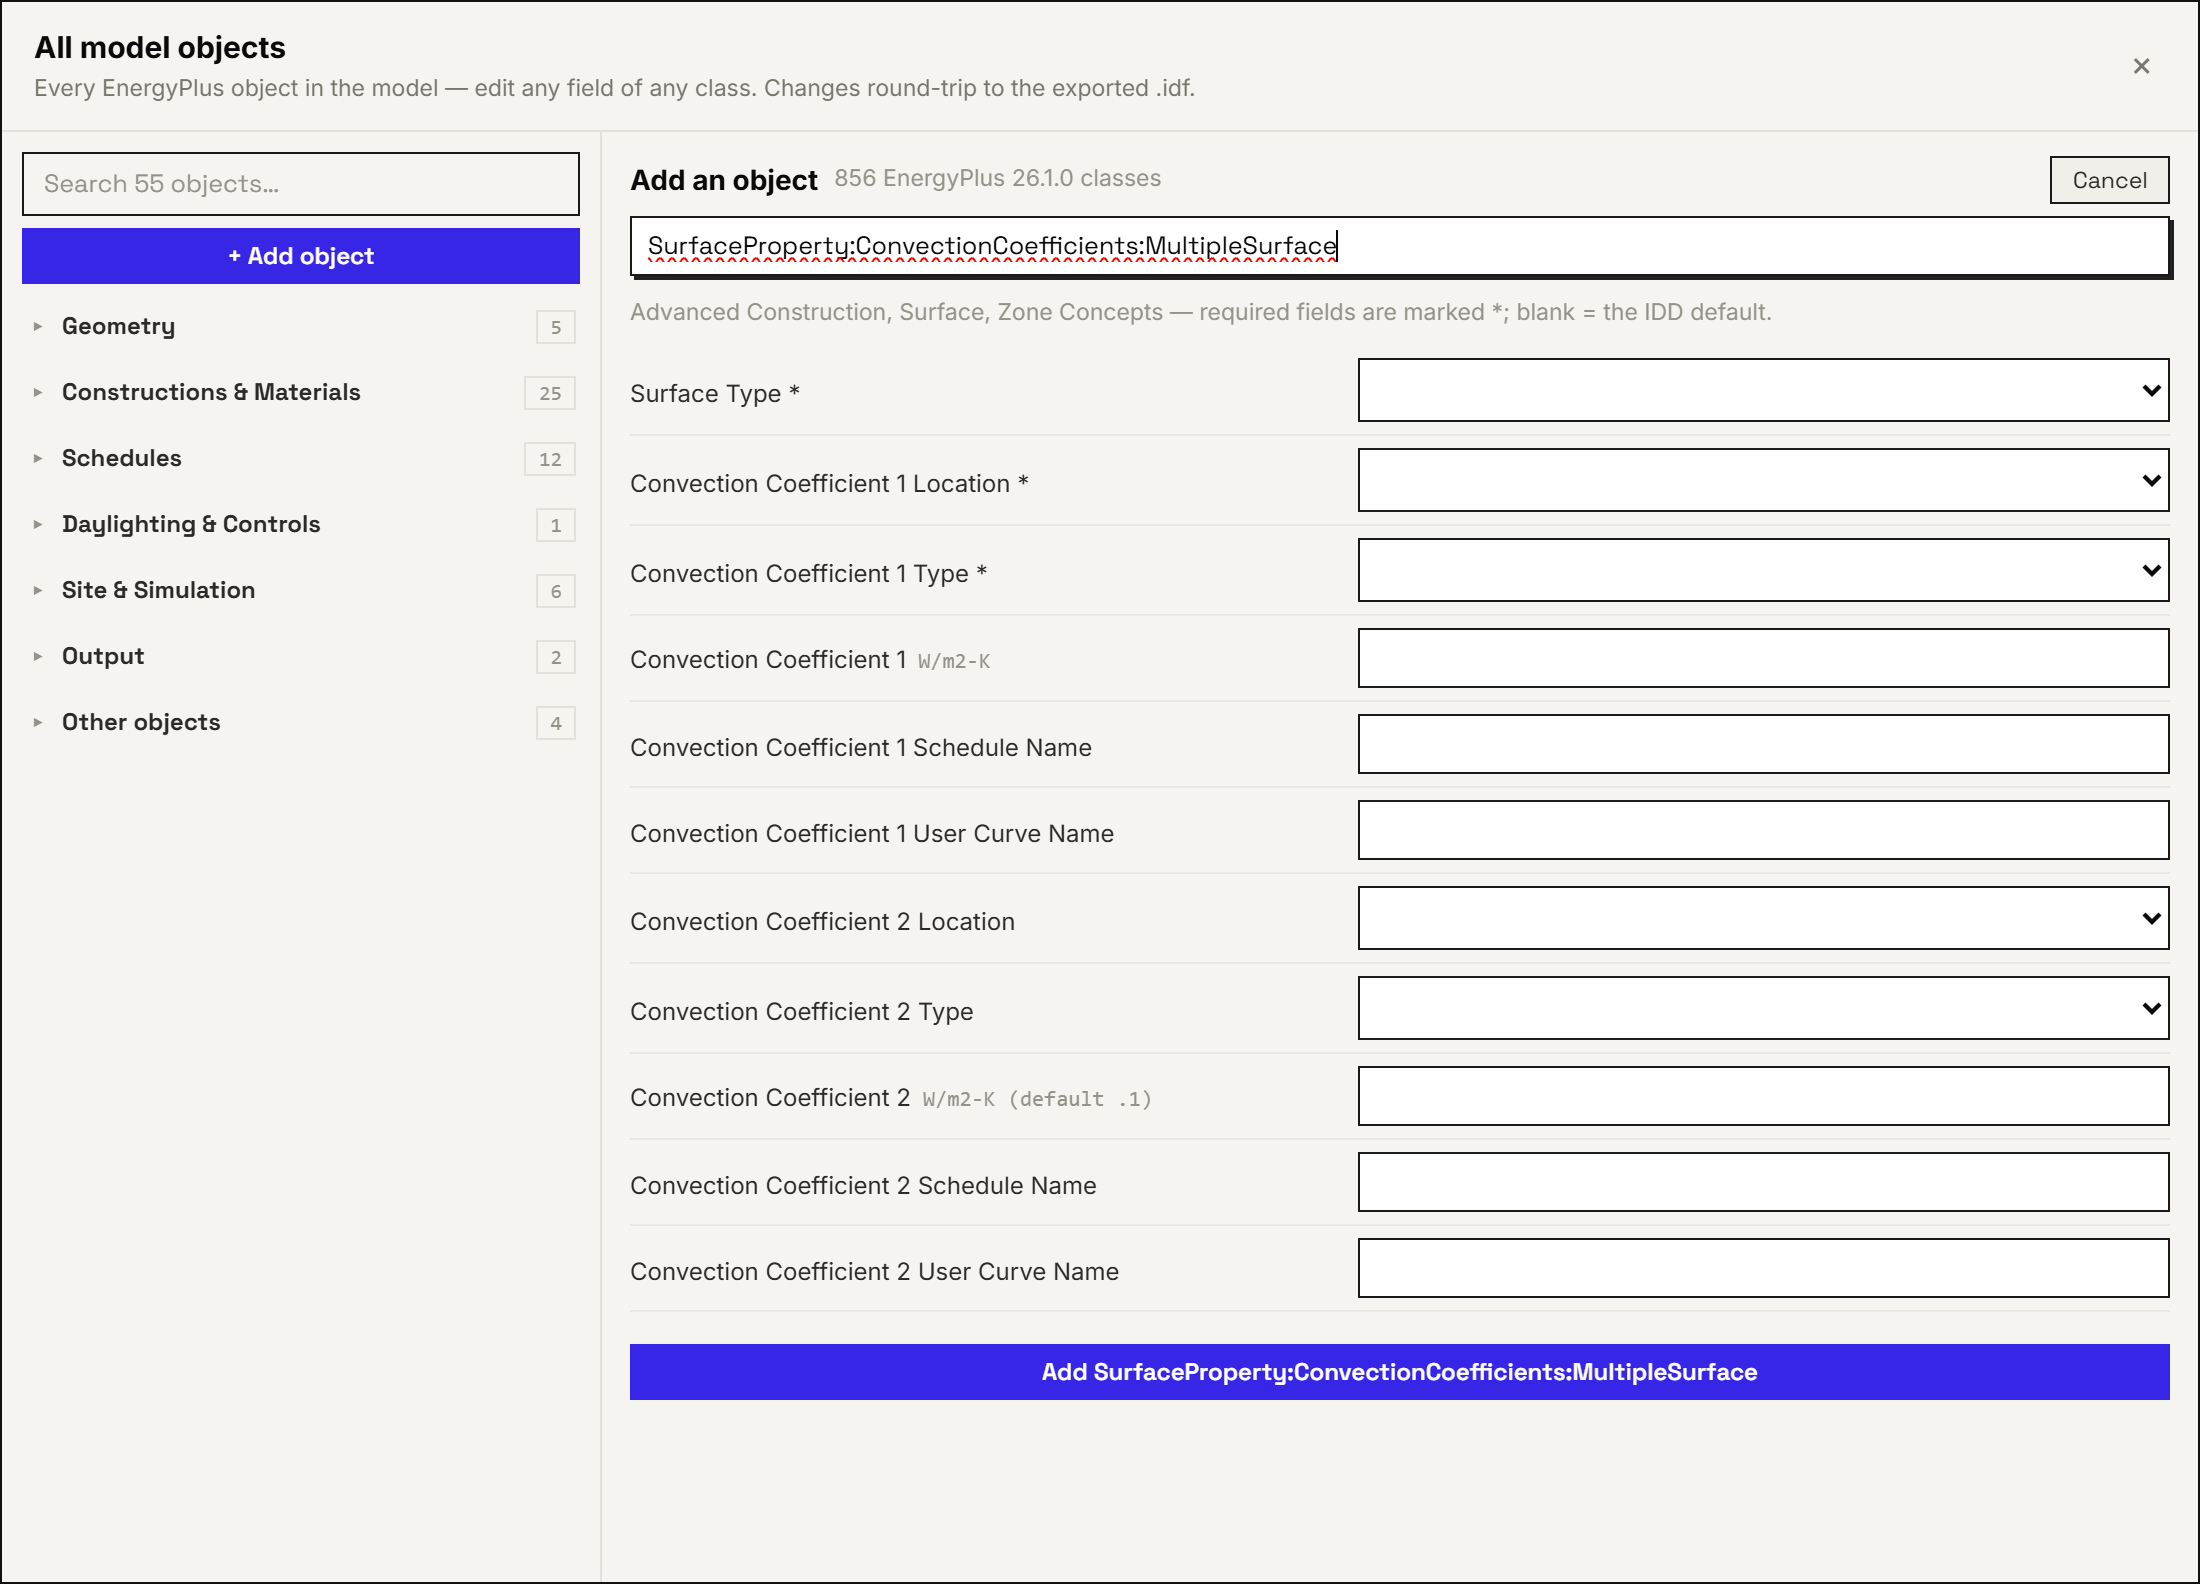
\includegraphics[height=4.1cm]{figures/ui/ui_add_object.png}}\hfil
\subfloat[Case~610 full-wall overhang in 3-D.\label{fig:shade}]{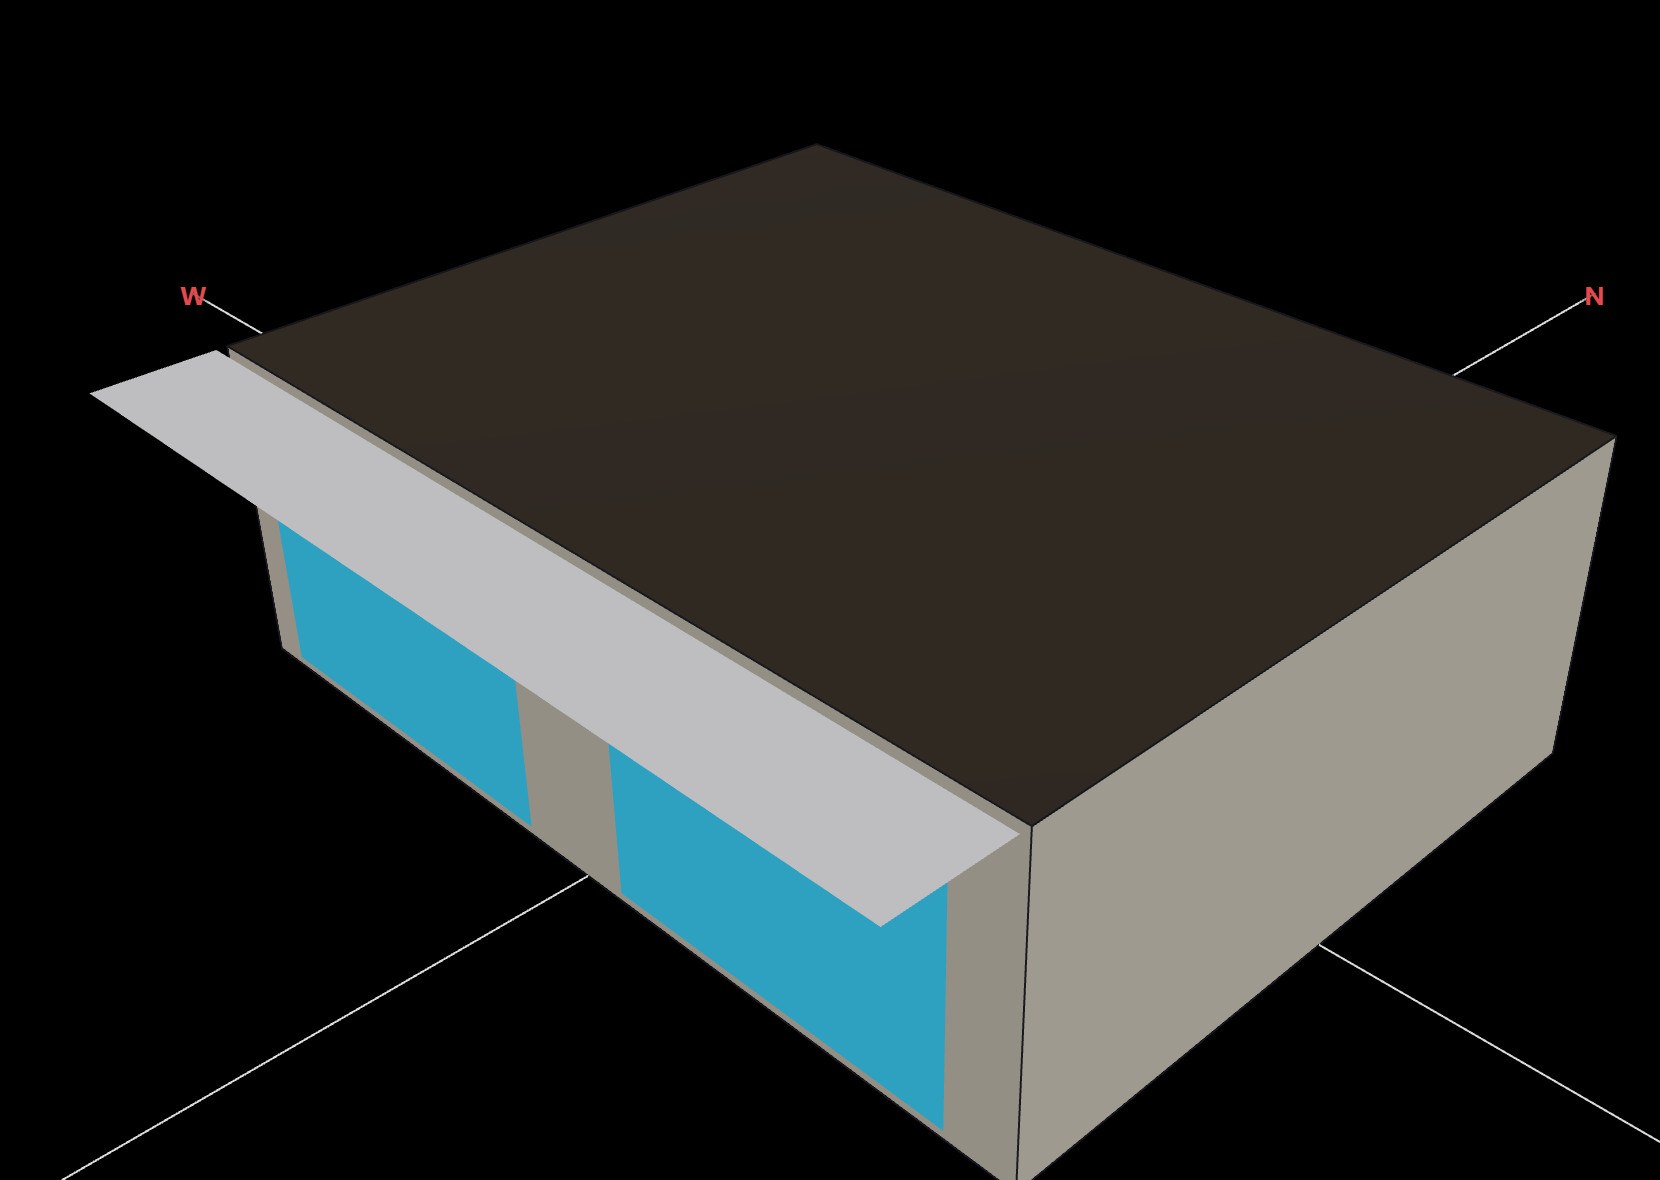
\includegraphics[height=4.1cm]{figures/ui/ui_shading_3d.png}}
\caption{Input-side interface features of the tested release that carry Standard~140 inputs (Sections 6--7).}\label{fig:ui1}
\end{figure*}

\begin{figure*}[!t]\centering
\subfloat[Kiva ground coupling (Section~8).\label{fig:kiva}]{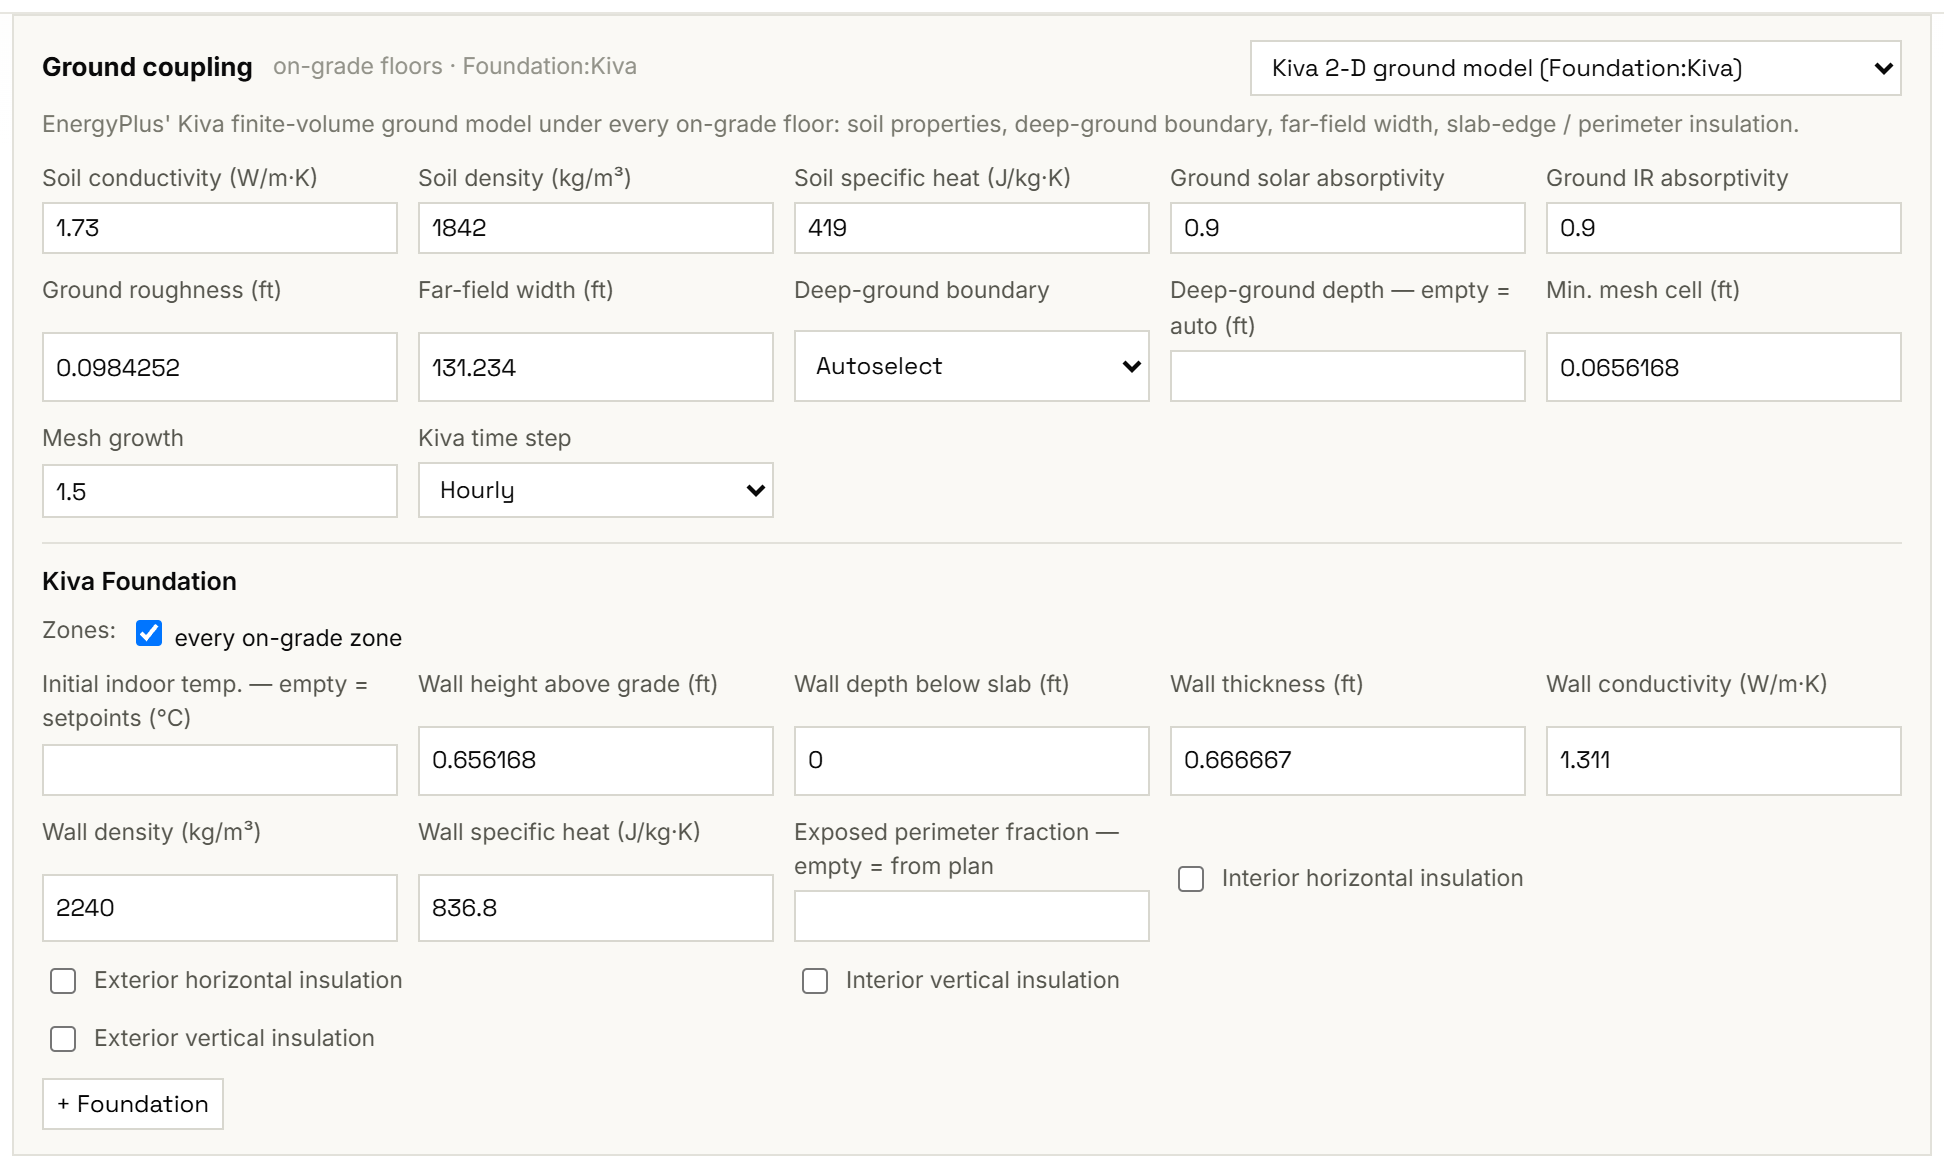
\includegraphics[height=3.6cm]{figures/ui/ui_ground_kiva.png}}\hfil
\subfloat[DX coil performance-map fitting, CE100 map (Section~9).\label{fig:dx}]{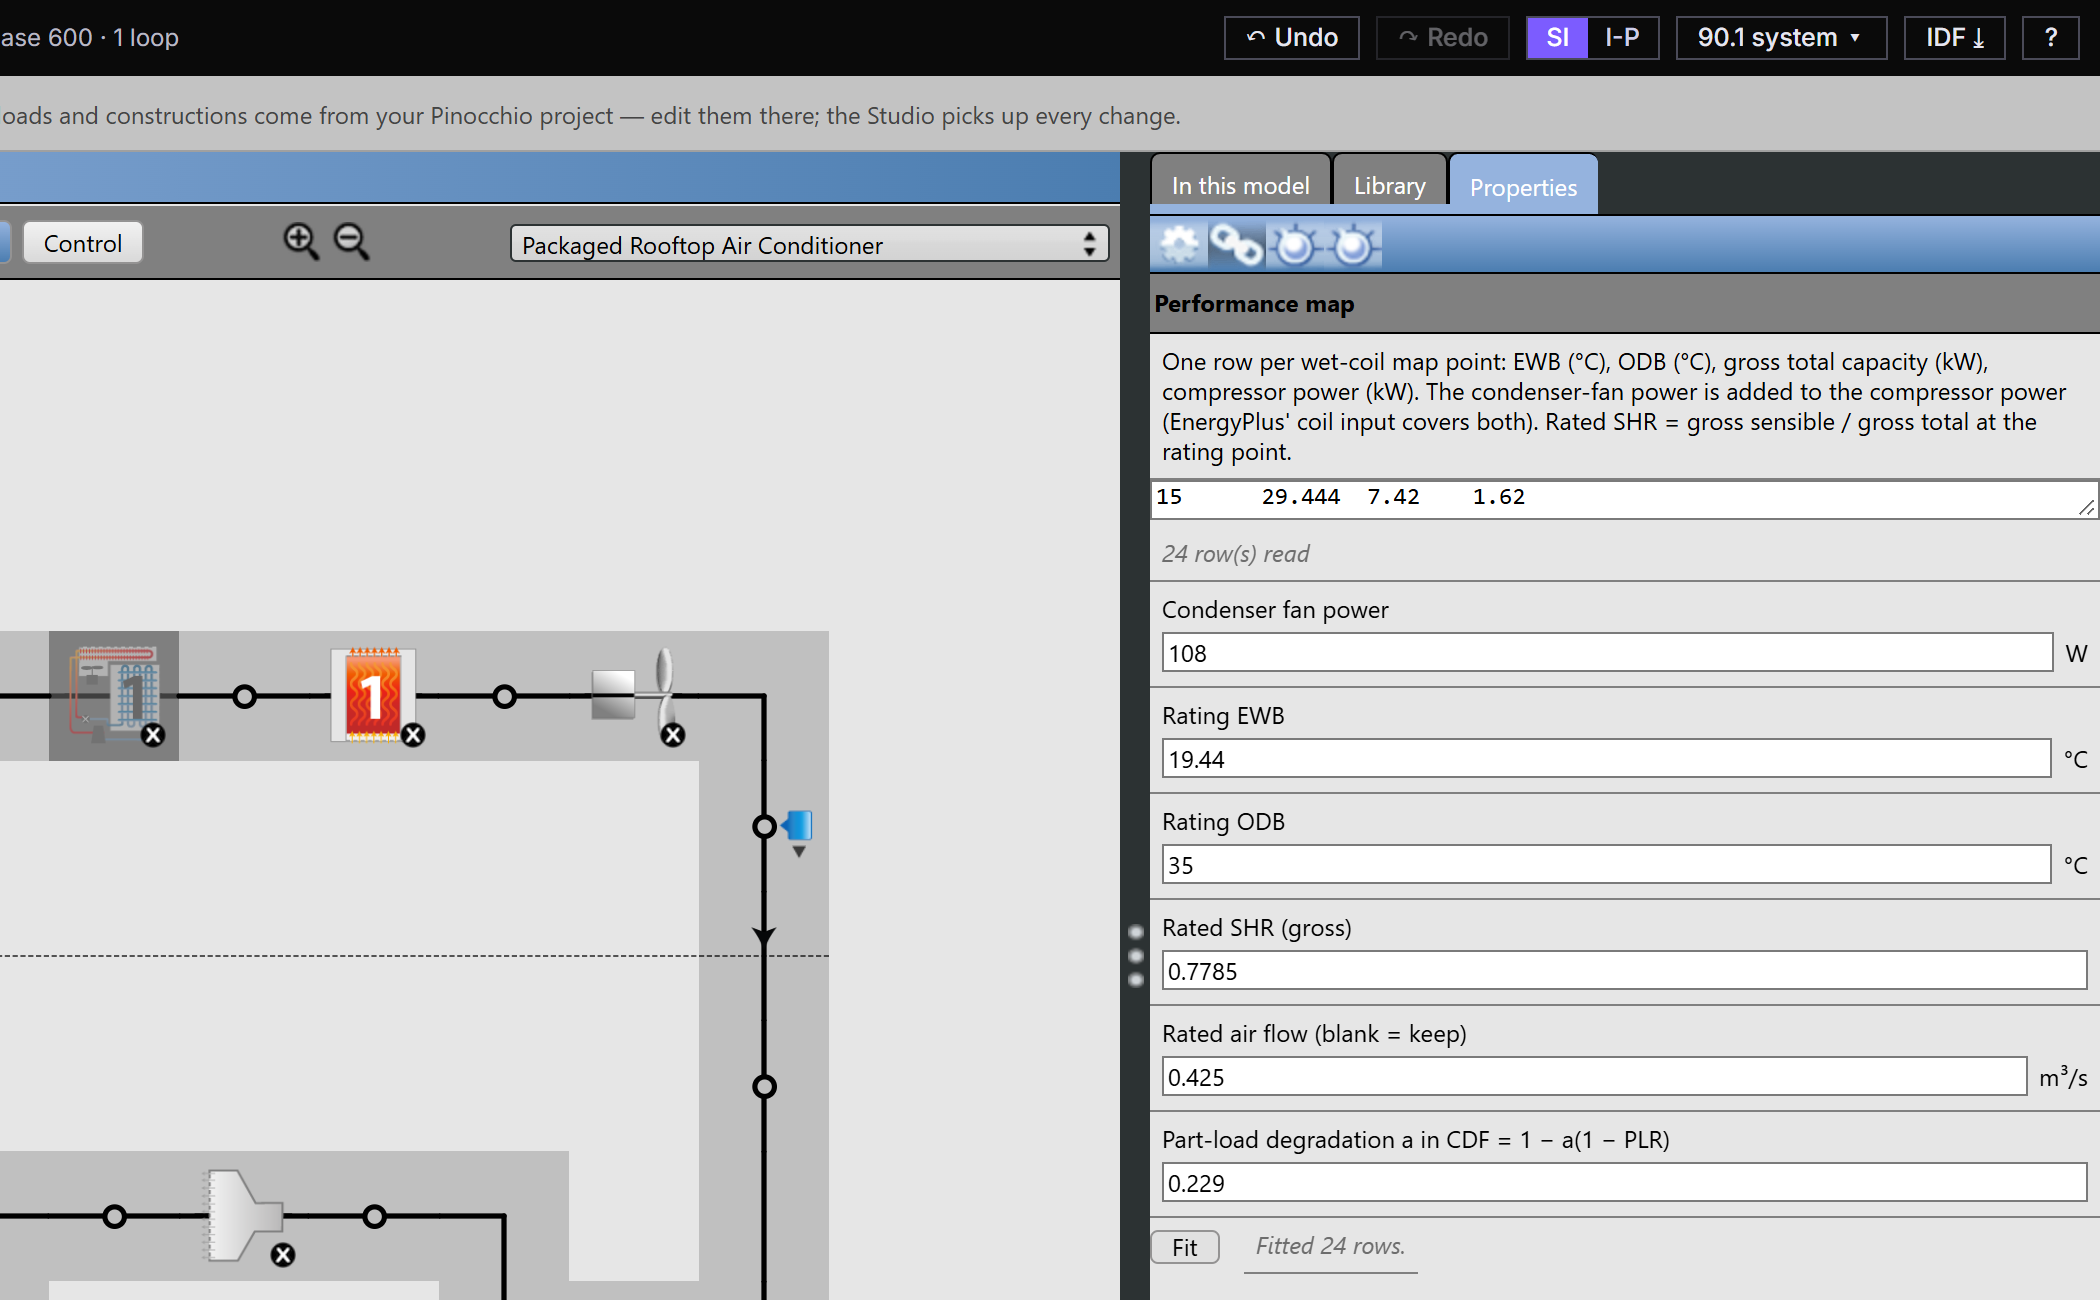
\includegraphics[height=3.6cm]{figures/ui/ui_studio_dxmap.png}}\hfil
\subfloat[Other-side-coefficient boundary (Section~13 guards).\label{fig:osc}]{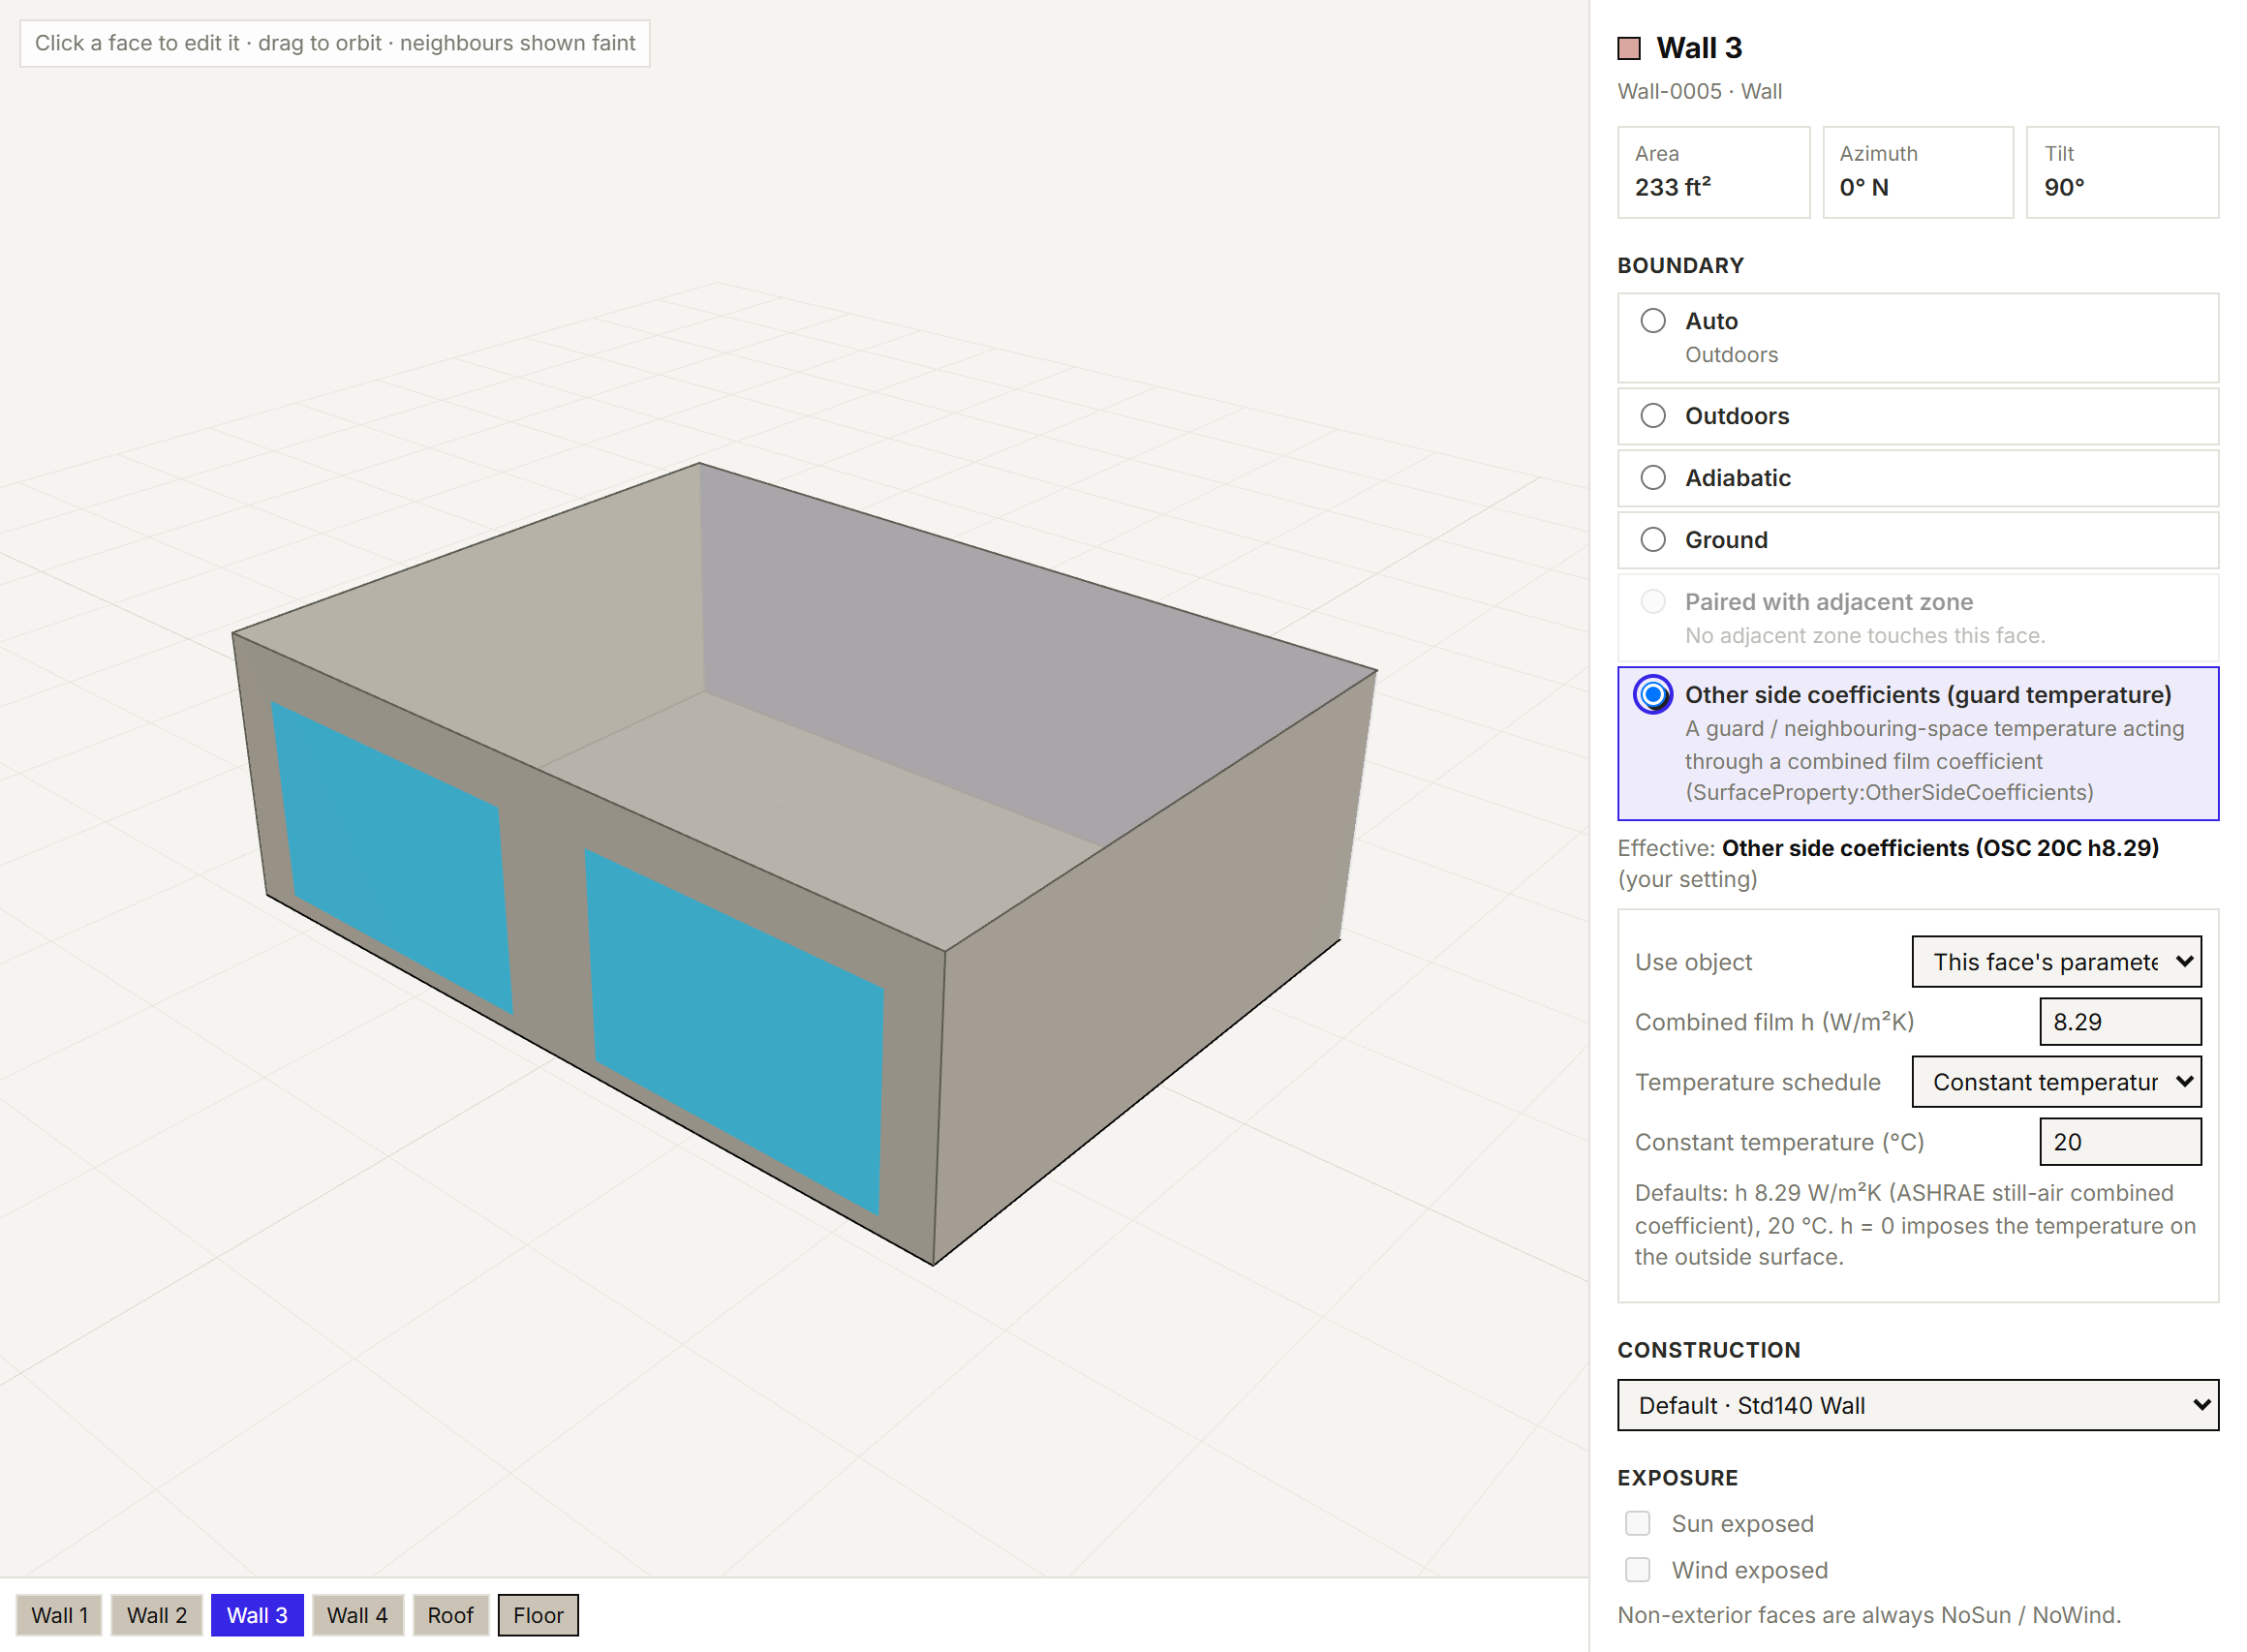
\includegraphics[height=3.6cm]{figures/ui/ui_surface_osc.png}}\\[2pt]
\subfloat[Results: raw ideal loads with timestamped peaks and the Std~140 report export (Case~600 run).\label{fig:res}]{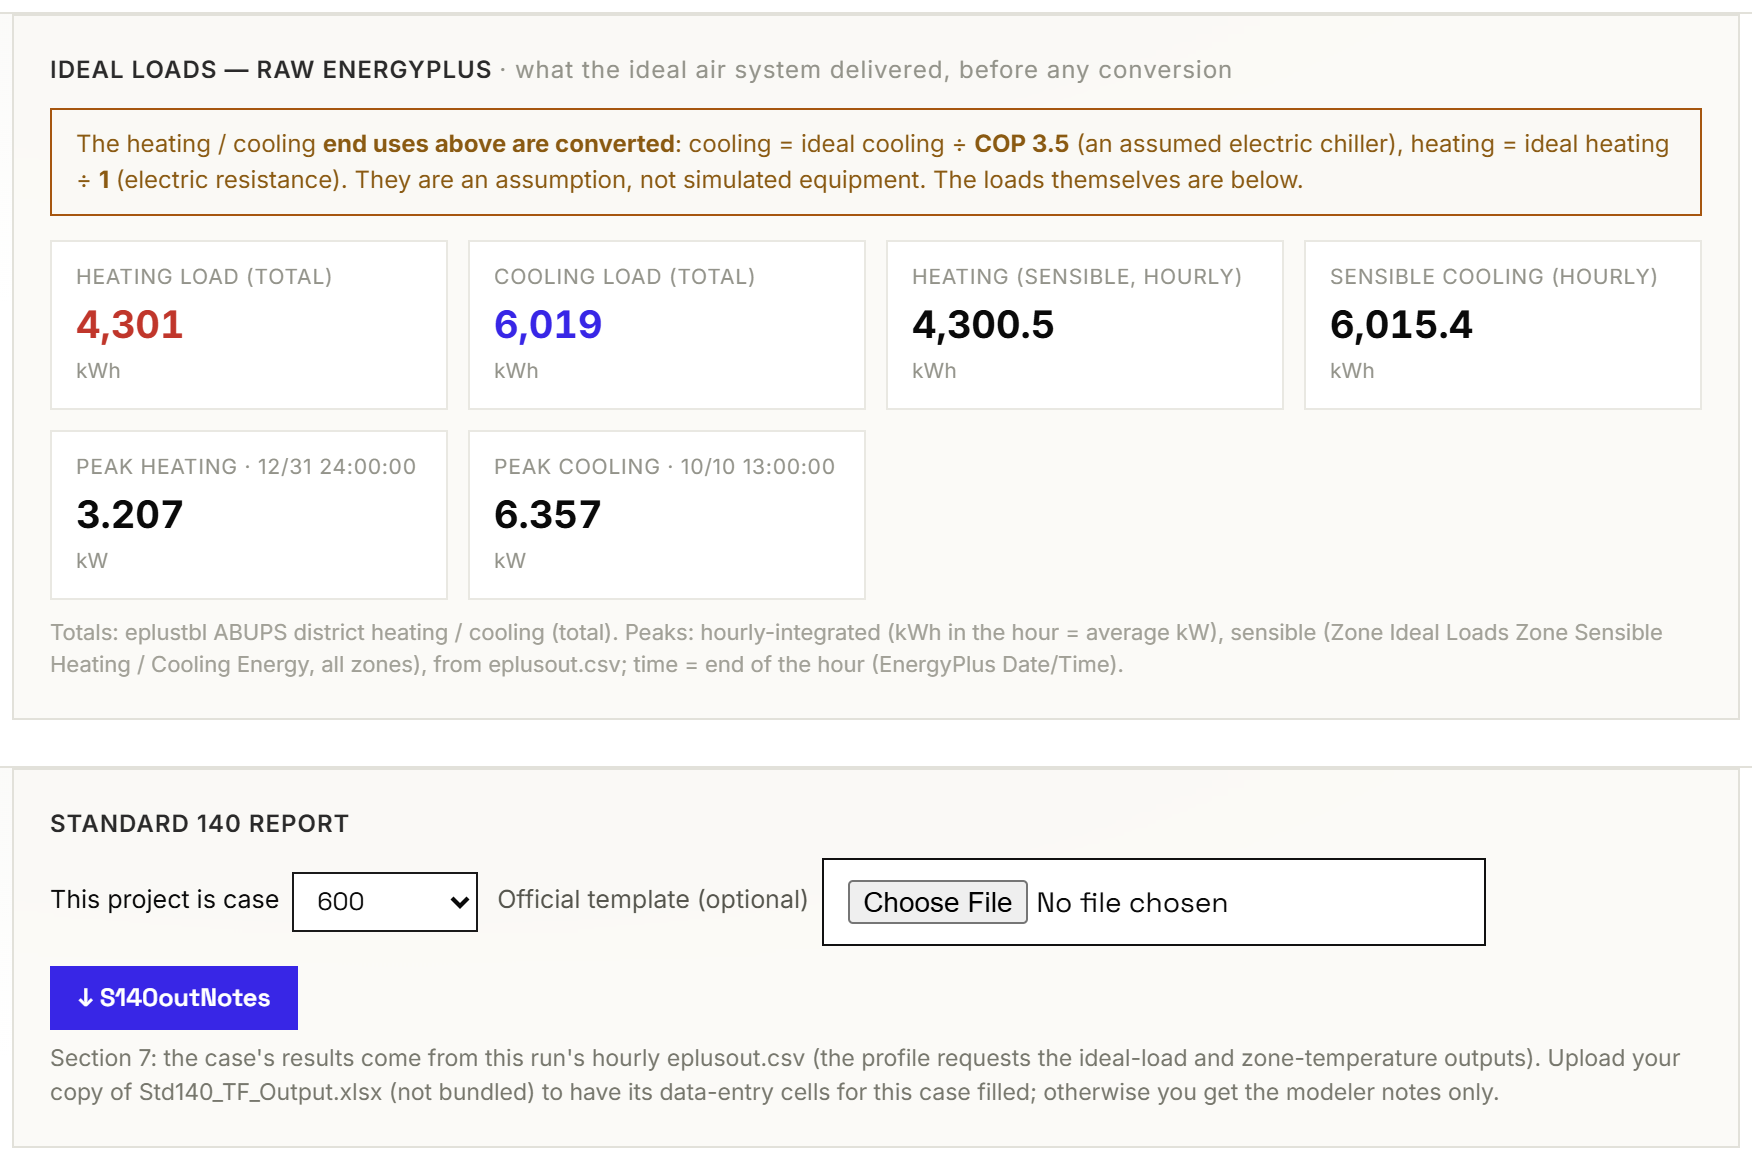
\includegraphics[height=5.0cm]{figures/ui/ui_results_std140.png}}\hfil
\subfloat[Review: profile notice; the model's own time step is used unaltered.\label{fig:rev}]{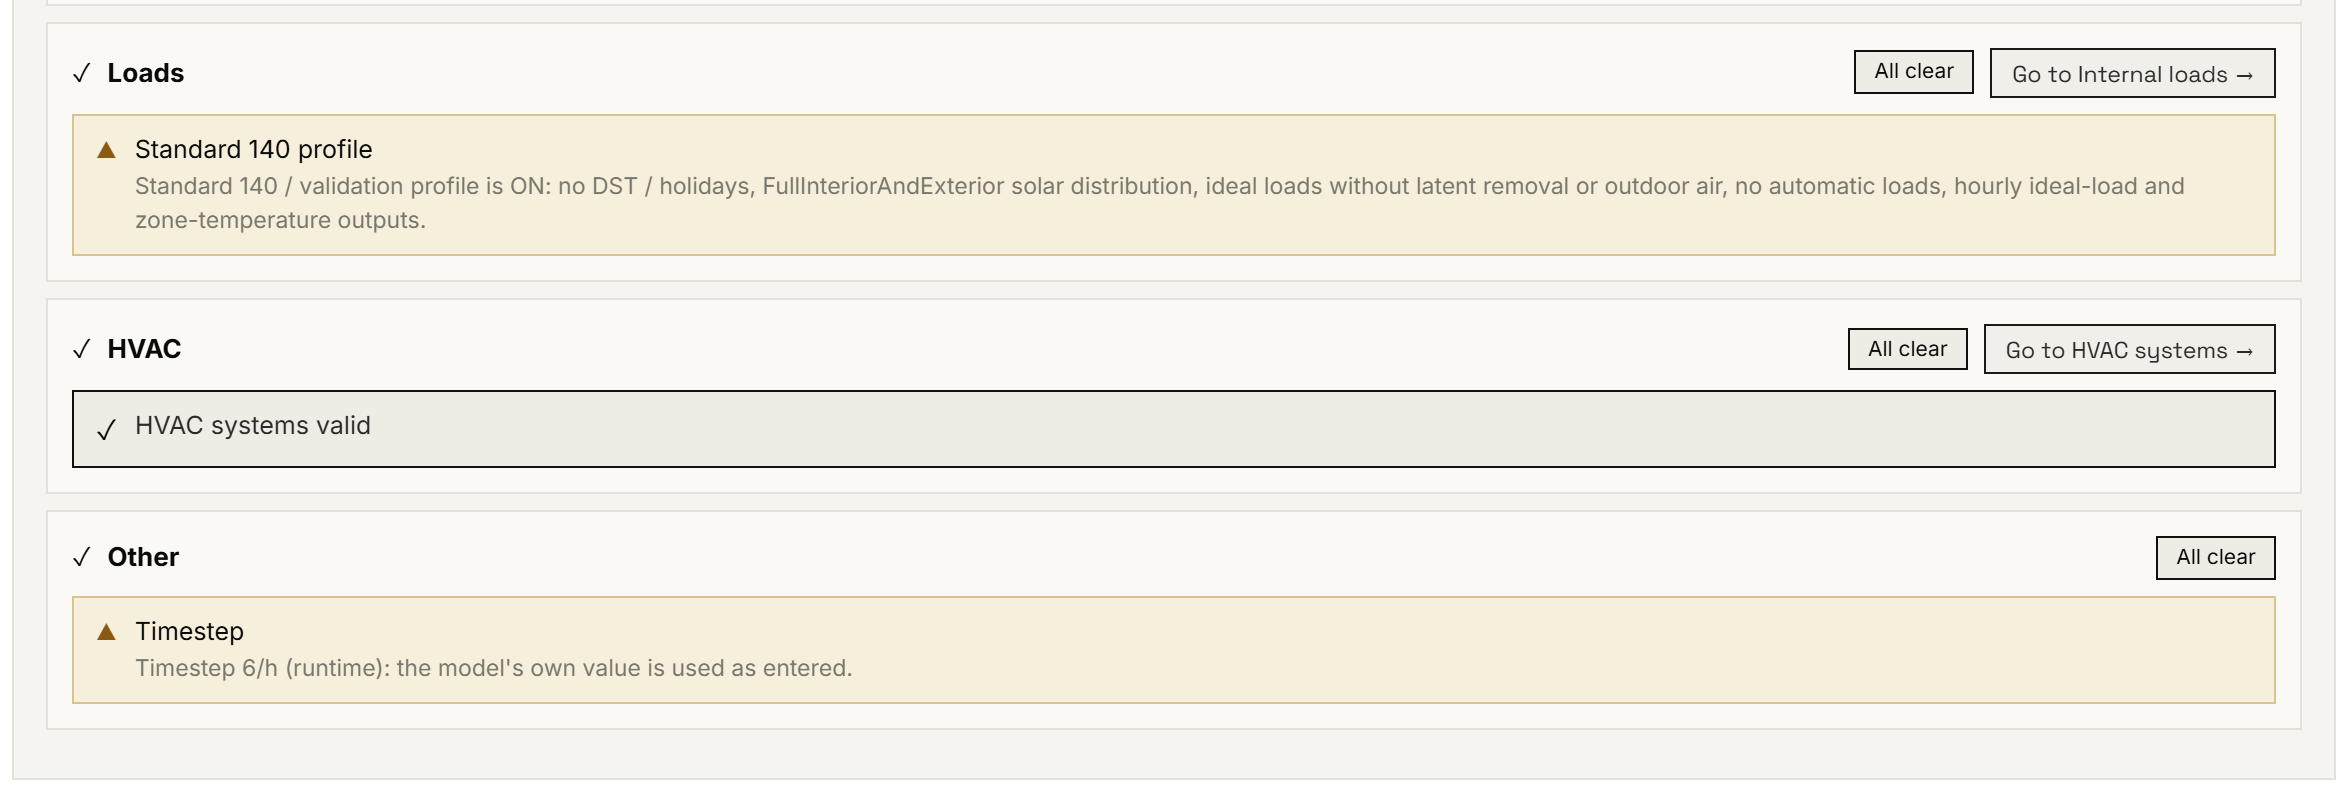
\includegraphics[width=0.42\textwidth]{figures/ui/ui_review_warnings.png}}
\caption{System, boundary, output and validation features (Sections 8--13, Annex A2).}\label{fig:ui2}
\end{figure*}

\begin{table}[!t]\centering\footnotesize
\caption{Standard Requirement to Implementation}\label{tab:map}
\begin{tabular}{@{}p{0.36\columnwidth}p{0.56\columnwidth}@{}}\toprule
Requirement & Pinocchio-EP implementation\\\midrule
Engine + UI tested together (A3) & every case through \code{exportIdf}\\
Time convention, no DST (5.1.1.1) & validation profile\\
Consistent numerics (5.1.1.4, 5.1.1.9) & time step never altered; shown in Review\\
Documented equivalent inputs (5.1.1.5) & S140outNotes block C\\
Weather formats (Sec.~6, A1) & TMY3/TMY2/TMY/WYEC2 converters\\
Envelope inputs (Sec.~7) & layered glazing, exact materials, shading\\
Constant coefficients (7.2.3) & convection panel\\
Ground coupling (Sec.~8) & Kiva panel\\
Equipment maps (Sec.~9--10) & map fitting, lookup part-load curves\\
Air systems (Sec.~11) & Studio: FC, SZ, CV and VAV reheat\\
Measured boundaries (Sec.~13) & other-side coefficients, schedule import\\
Outputs (7.3, A2) & output picker, peaks, report export\\
Version identifier (A2 block A) & build stamp in UI and IDF\\\bottomrule
\end{tabular}\end{table}

\section{Limitations and External Defects}\label{sec:limits}
\begin{itemize}
\item \textbf{Section~8:} GC10a cannot be represented in Kiva, which is two-dimensional and has no ground-temperature
output points.
\item \textbf{Section~12:} the results show a low bias in the window-related terms; its cause is under
investigation.
\end{itemize}
Defects found in EnergyPlus~26.1, all reported and none patched:
\begin{itemize}
\item the FisherPedersen ceiling-diffuser keys are fatal in \code{MultipleSurface};
\item the economizer lockout is ignored on load-controlled unitary systems;
\item economizer-first staging crashes the engine;
\item the EPW albedo column is ignored;
\item wind direction is interpolated straight through north.
\end{itemize}
Defects found in the standard's own files, all handled and documented:
\begin{itemize}
\item an equation-of-time typo in A1.5;
\item an inconsistent WD400 header;
\item a TMY local-standard-time offset;
\item a duplicated WYEC2 hour stamp.
\end{itemize}

\section{Conclusion}
The tested release of Pinocchio-EP passes every graded test group of ANSI/ASHRAE Standard~140-2023, with
Addendum~a's time-series criteria, using ASHRAE's official files. It also reproduces Addendum~b's measured heater
energy to within the measurement uncertainty. The result rests on documented practices: a pinned, unmodified
engine; inputs that are never silently altered; standard-format reporting; versioned builds; automated regression
against Annex~A3. The full suite was generated on build \code{1.0.0+b7b2379}. The deployed release
\code{1.0.0+e2c8ebf} changes only a Review display card; the on-engine Annex~A3 regression gate and all 992 tests
were re-run on it. Future releases are re-tested by the same harness.

\begin{thebibliography}{10}
\bibitem{s140} \emph{Method of Test for Evaluating Building Performance Simulation Software}, ANSI/ASHRAE Standard 140-2023, ASHRAE, Peachtree Corners, GA, USA, 2023.
\bibitem{s140a} \emph{Addendum a to ANSI/ASHRAE Standard 140-2023}, ANSI/ASHRAE/IBPSA, Aug. 2025.
\bibitem{s140b} \emph{Addendum b to ANSI/ASHRAE Standard 140-2023}, ANSI/ASHRAE/IBPSA, Apr. 2026.
\bibitem{s140files} ASHRAE, ``Standard 140-2023 accompanying files,'' [Online]. Available: \url{https://data.ashrae.org/standard140/}
\bibitem{s901} \emph{Energy Standard for Sites and Buildings Except Low-Rise Residential Buildings}, ANSI/ASHRAE/IES Standard 90.1-2022, ASHRAE, 2022.
\bibitem{eplus} U.S. Department of Energy, \emph{EnergyPlus Version 26.1.0 Documentation}, 2026. [Online]. Available: \url{https://energyplus.net}
\bibitem{osstd} National Renewable Energy Laboratory, ``openstudio-standards,'' v0.8.5. [Online]. Available: \url{https://github.com/NREL/openstudio-standards}
\bibitem{kiva} N. Kruis and M. Krarti, ``Kiva\texttrademark: A numerical framework for quickly modeling ground-coupled heat transfer,'' \emph{J. Building Performance Simulation}, vol. 10, no. 5--6, 2017.
\bibitem{tmy3} S. Wilcox and W. Marion, ``Users manual for TMY3 data sets,'' NREL, Golden, CO, USA, Tech. Rep. NREL/TP-581-43156, 2008.
\bibitem{etna} ETNA test facility (EDF R\&D), as specified in Addendum~b to ASHRAE Standard 140-2023, Section~13.
\bibitem{doe179d} U.S. Department of Energy, ``Qualified software for calculating commercial building tax deductions,'' [Online]. Available: \url{https://www.energy.gov/eere/buildings/qualified-software-calculating-commercial-building-tax-deductions}
\end{thebibliography}
\end{document}
